\input ../SlidePreamble
\input ../preamble

\begin{document}

{\Huge
  
  \centerline{\bf TTIC 31230, Fundamentals of Deep Learning}
  \bigskip
  \centerline{David McAllester, Winter 2019}
  \vfill
  \vfill
  \centerline{\bf Deep Learning Frameworks}
  \vfill
  \vfill

\slideplain{What is a Deep Learning Framework?}

A framework provides a high level language for writing models $P_\Phi(y|x)$.

\vfill
A framework compiles a model into an optimization algorithm.
\vfill
{\color{red} $$\Phi^* \approx \argmin_\Phi E_{(x,y) \sim \mathrm{Train}} \; -\ln P_\Phi(y|x)$$}

\vfill
A framework also typically provides support for managing large training sets and pre-trained model parameter values (also called ``models'').

\slide{Some Frameworks}

\begin{itemize}
  
\item Kaffe

\vfill

\item Tensorflow

\vfill

\item DyNet

  \vfill
\item Chainer

\vfill

\item PyTorch

  \vfill

\item EDF (Educational Framework in Python for this class).
\end{itemize}

$\vdots$

\slide{An Example: Multi-Layer Perceptron Models for MNIST}

We consider the problem of taking an input $x$ (such as an image of a hand written digit) and classifying it into some small number of classes (such as the digits $0$ through $9$).

\vfill
\centerline{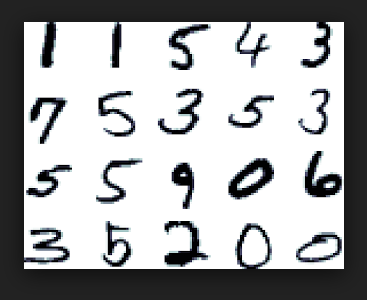
\includegraphics[width= 4.0in]{../images/MNIST}}
  
\slide{Multiclass Classification}

Assume a population distribution on pairs $(x,y)$ for $x \in \reals^d$ and $y \in \{y_1,\ldots, y_k\}$.

\vfill
For MNIST $x$ is a $28 \times 28$ image which we take to be a 784 dimensional vector giving $x \in \reals^{784}$.

\vfill
For MNIST $k = 10$.

\vfill
Let $\mathrm{Train}$ be a sample $(x_0,y_0),\;\ldots,\;(x_{N-1},y_{N-1})$ drawn IID from the population.

\slide{A Multi Layer Perceptron (MLP)}

$$\Phi = (W^0,\;b^0,\;W^1,\;b^1)$$

\begin{eqnarray*}
  {\color{red} h} & = & \sigma\left(W^0{\color{red} x} - b^0\right) \\
  \\
  {\color{red} s} & = & \sigma\left(W^1{\color{red} h} - b^1 \right) \\
  \\
  {\color{red} P_\Phi[\hat{y}]} & = & \softmax_{\hat{y}}\;{\color{red} s[\hat{y}]}
\end{eqnarray*}

\slide{Activation Functions}

An activation function $\sigma:\reals \rightarrow \reals$ (scalar-to-scalar) is applied to each component of a vector.

\vfill
\centerline{{\color{red} $\sigma(u) = \frac{1}{1+e^{-u}}$}\hspace{3em}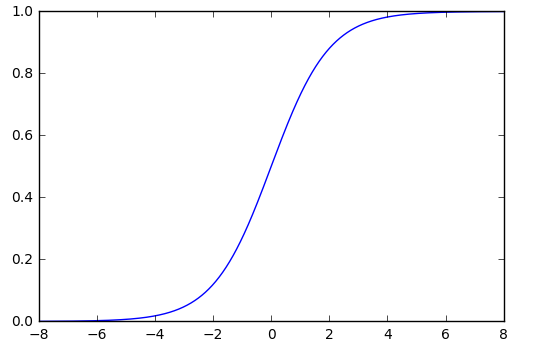
\includegraphics[width=1.5in]{../images/sigmoid}, {\color{red} $\sigma(m) = P(y|m)$ for margin $m$}.}

\vfill
other common activation functions are

\vfill
\centerline{{\color{red} $\mathrm{ReLU}(u) = \max(0,u)$}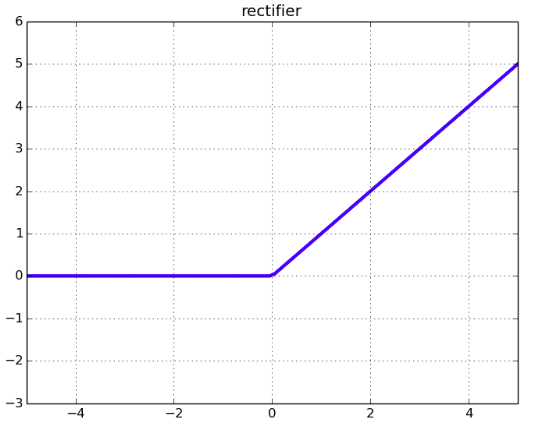
\includegraphics[width=1.5in]{../images/relu},
{\color{red} $\mathrm{tanh}(u) = 2\sigma(u)-1$}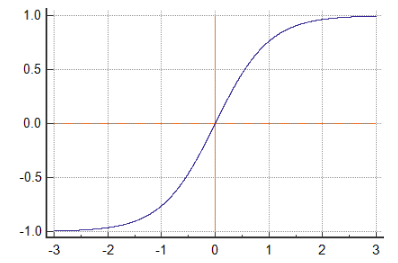
\includegraphics[width=1.5in]{../images/tanh}}

\slide{Einstein Notation}

$${\color{red} h} = \sigma\left(W^0{\color{red} x} - b^0\right)$$

\vfill
is an abbreviation for
\begin{eqnarray*}
  {\color{red} h[j]} & = & \sigma\left(\left(\sum_i\;W^0[j,i] \;{\color{red} x[i]}\right) - b^0[j]\right) 
\end{eqnarray*}

\vfill
Think of this as a separate assignment statement for each {\color{red} $j$}.

\vfill
Each {\color{red} $h[j]$} is the output of a ``linear threshold unit''.

\vfill
Einstein notation makes all indeces and summations explicit.

\slide{Optimization}

Once we have specified our model $P_\Phi(y|x)$ in high level equations (such as on the previous two slides) we need to train it.

$$\Phi^* \approx \argmin_\Phi E_{(x,y) \sim {\color{red} \mathrm{Train}}} \; - \ln P_\Phi(y|x)$$

\vfill
The framework generates the training code automatically from the model definition.

\vfill
{\color{red} Optimization is almost always done with some form of stochastic gradient descent (SGD) and the gradient is computed
by back-propagation on the model definition.}

\slide{Stochastic Gradient Descent (SGD)}
$$\Phi^* = \argmin_\Phi E_{(x,y) \sim \mathrm{Train}} \; {\cal L}(x,y,\Phi).$$

\vfill
\begin{enumerate}
\item Randomly Initialize $\Phi$ (initialization is important and must be done with care).

  \vfill
  \item Repeat until ``converged'':

    \vfill
    \begin{itemize}
    \item draw $(x,y) \sim \mathrm{Train}$ at random.
      \vfill
    \item $\Phi \;\;\minuseq\;\; \eta \nabla_\Phi\;{\cal L}(x,y,\Phi)$
    \end{itemize}
\end{enumerate}

\slide{Epochs}

In practice we cycle through the training data visiting each training pair once.

\vfill
One pass through the training data is called an Epoch.

\vfill
One typically imposes a random suffle of the training data before each epoch.

\slide{SGD for MLPs}

$$\Phi = (W^0,\;b^0,\;W^1,\;b^1)$$

\begin{eqnarray*}
  {\color{red} h} & = & \sigma\left(W^0{\color{red} x} - b^0\right) \\
  \\
  {\color{red} s} & = & \sigma\left(W^1{\color{red} h} - b^1 \right) \\
  \\
  {\color{red} P_\Phi[\hat{y}]} & = & \softmax_{\hat{y}}\;{\color{red} s[\hat{y}]}
\end{eqnarray*}

\vfill
We now need to automatically compute $\nabla_\Phi {\cal L}(x,y,\Phi)$.



\ignore{
\slide{Total Gradient Descent}

$${\cal L}_{\mathrm{Train}}(\Phi) = \frac{1}{N}\sum_n {\cal L}(\Phi,x_n,y_n)$$

\vfill
\centerline{We want: \hspace{3ex} $\Phi^*  =  \argmin_\Phi {\cal L}_{\mathrm{Train}}(\Phi)$}

\vfill
$$\Phi \;\;\;\mbox{\tt -=}\;\;\; \eta \nabla_\Phi {\cal L}_\mathrm{Train}(\Phi)$$


\slide{Stochastic Gradient Descent (SGD) on the Training set.}

\vfill
\vfill
repeat:  Select $n$ at random. $\Phi \;\;\minuseq\;\; \eta \;\nabla_\Phi \; {\cal L}(x_n,y_n,\Phi)$

\begin{eqnarray*}
  \expectsub{n}{\nabla_\Phi \; {\cal L}(x_n,y_n,\Phi)} & = & \sum_n P(n) \nabla_\Phi\;{\cal L}_{\mathrm{Train}}(x_n,y_n,\Phi) \\
  \\
  \\ & = & \frac{1}{N} \sum_n \nabla_\Phi\;{\cal L}_{\mathrm{Train}}(x_n,y_n,\Phi) \\
  \\
    \\ & = & \nabla_\Phi \frac{1}{N} \sum_n \;{\cal L}_{\mathrm{Train}}(x_n,y_n,\Phi) \\
  \\
  &  = & \nabla_\Phi\;{\cal L}_{\mathrm{Train}}(\Phi)
\end{eqnarray*}
}

\slideplain{Computation Graphs (Framework Source Code)}

A computation graph (sometimes called a ``computation{\color{red} al} graph'') is a sequence of assignment statements.


\begin{eqnarray*}
  {\color{red} h} & = & \sigma\left(W^0{\color{red} x} - b^0\right) \\
  \\
  {\color{red} s} & = & \sigma\left(W^1{\color{red} h} - b^1 \right) \\
  \\
  {\color{red} P_\Phi[\hat{y}]} & = & \softmax_{\hat{y}}\;{\color{red} s[\hat{y}]}
\end{eqnarray*}

\vfill
I prefer the term ``source code'' to the term ``graph''.

\slideplain{Simpler Source Code}

The expression

\vfill
{\color{red} $${\cal L} = \sqrt{x^2 + y^2}$$}

\vfill
can be transformed to the assignment sequence

{\color{red}
\vfill
\begin{eqnarray*}
  u & = & x^2  \\
  v & = & y^2 \\
  r & =& u + v \\
  {\cal L} & = & \sqrt{r}
\end{eqnarray*}
}

\anaslide{Source Code}
\vspace{-1ex}
{\color{red}
$$\begin{array}{lcl}
 1.\;u & = & x^2  \\
 2.\;w & = & y^2 \\
 3.\;r & =& u + w \\
  4.\;{\cal L} & = & \sqrt{r}
\end{array}$$
}

\vfill
For each variable $z$, the derivative $\partial {\cal L}/\partial z$ will get computed in reverse order.

\vfill
{\color{red}
$$\begin{array}{lcl}
(4)\; \partial{\cal L}/\partial r & = & \frac{1}{2\sqrt{r}} \\
(3)\; \partial{\cal L}/\partial u & = & \partial {\cal L}/\partial r \\
(3)\; \partial{\cal L}/\partial w & = & \partial {\cal L}/\partial r\\
(2)\; \partial{\cal L}/\partial y & = &  (2y) * (\partial {\cal L}/\partial w) \\
(1)\; \partial{\cal L}/\partial x & = & (2x) * (\partial {\cal L}/\partial u)
\end{array}$$
}

\anaslideplain{A More Abstract Example (Still Scalar Values)}
\vspace{-3ex}
\begin{eqnarray*}
  y & = & f(x) \\
  z & = & g(y,x) \\
  u & = & h(z) \\
  {\cal L} & = & u
\end{eqnarray*}

\medskip
For now assume all values are scalars (single numbers rather than arrays).

\medskip
We will ``backpopagate'' the assignments the reverse order.

\anaslide{Back-Propagation (Scalar Values)}
\vspace{-3ex}
\begin{eqnarray*}
  y & = & f(x) \\
  z & = & g(y,x) \\
  u & = & h(z) \\
  {\cal L} &  = & {\color{red} u}
\end{eqnarray*}

\medskip
{\color{red} ${\partial {\cal L}}/{\partial u} = 1$}

\anaslide{Back-Propagation (Scalar Values)}
\vspace{-3ex}
\begin{eqnarray*}
  y & = & f(x) \\
  z & = & g(y,x) \\
  u & = & h({\color{red} z}) \\
  {\cal L} &  = &  u
\end{eqnarray*}

\medskip
${\partial {\cal L}}/{\partial u} = 1$

\medskip
{\color{red} ${\partial {\cal L}}/{\partial z} = ({\partial h}/{\partial z})\; ({\partial {\cal L}}/{\partial u})$} (this uses the value of $z$)

\anaslide{Back-Propagation (Scalar Values)}
\vspace{-3ex}
\begin{eqnarray*}
  y & = & f(x) \\
  z & = & g({\color{red} y},x) \\
  u & = & h(z) \\
  {\cal L} &  = &  u
\end{eqnarray*}

\medskip
${\partial {\cal L}}/{\partial u} = 1$

\medskip
${\partial {\cal L}}/{\partial z} = ({\partial h}/{\partial z}) \; ({\partial {\cal L}}/{\partial u})$

\medskip
{\color{red} ${\partial {\cal L}}/{\partial y} = ({\partial g}/{\partial y}) \; ({\partial {\cal L}}/{\partial z})$} (this uses the value of $y$ and $x$)

\anaslide{Back-Propagation (Scalar Values)}
\vspace{-3ex}
\begin{eqnarray*}
  y & = & f({\color{red} x}) \\
  z & = & g(y,{\color{red} x}) \\
  u & = & h(z) \\
  {\cal L} &  = &  u
\end{eqnarray*}

\medskip
${\partial {\cal L}}/{\partial u} = 1$

\medskip
${\partial {\cal L}}/{\partial z} = ({\partial h}/{\partial z}) \;({\partial {\cal L}}/{\partial u})$

\medskip
${\partial {\cal L}}/{\partial y} = ({\partial g}/{\partial y}) \;({\partial {\cal L}}/{\partial z})$

\medskip
{\color{red} ${\partial {\cal L}}/{\partial x} =$ ???} Oops, we need to add up multiple occurrences.

\anaslide{Back-Propagation (Scalar Values)}
\vspace{-3ex}
\begin{eqnarray*}
  y & = & f({\color{red} x}) \\
  z & = & g(y,{\color{red} x}) \\
  u & = & h(z) \\
  {\cal L} &  = &  u
\end{eqnarray*}

\medskip
Each framework program variable denotes an {\color{red} object} (in the sense of C++ or Python).

\medskip
{\color{red} $x.\mathrm{value}$} and {\color{red} $x.\grad$} are attributes of the {\color{red} object $x$}.

\bigskip
Values are computed ``forward'' while gradients are computed ``backward''.


\anaslide{Back-Propagation (Scalar Values)}
\vspace{-3ex}
\begin{eqnarray*}
  y & = & f(x) \\
  z & = & g(y,x) \\
  u & = & h(z) \\
  {\color{red} {\cal L}} &  {\color{red} =} & {\color{red}  u}
\end{eqnarray*}


\bigskip
We initialize {\color{red} $x.\mathrm{grad}$} to zero: {\color{red} $z.\grad = y.\grad = x.\grad = 0$}

\bigskip
We initialize the loss gradient to 1: {\color{red} $u.\grad = 1$}

\medskip
{\bf Loop Invariant}: For any variable $w$ whose definition has not yet been processed we have that $w.\grad$ is $\partial {\cal L}/\partial w$ as defined by the set of assignments already processed.

\anaslide{Back-Propagation (Scalar Values)}
\vspace{-3ex}
\begin{eqnarray*}
  y & = & f(x) \\
  z & = & g(y,x) \\
  {\color{red} u} & {\color{red} =} & {\color{red} h(z)} \\
  {\color{red} {\cal L}} & {\color{red}  =} &  {\color{red} u}
\end{eqnarray*}

{\color{red}
\medskip
$z.\grad = y.\grad = x.\grad = 0$

\medskip
$u.\grad = 1$

\medskip
$z.\grad\;\pluseq\;  ({\partial h}/{\partial z}) * u.\grad$

}

\medskip
{\bf Loop Invariant}: For any variable $w$ whose definition has not yet been processed we have that $w.\grad$ is $\partial {\cal L}/\partial w$ as defined by the set of assignments already processed.

\anaslide{Back-Propagation (Scalar Values)}
\vspace{-3ex}
\begin{eqnarray*}
  y & = & f(x) \\
  {\color{red} z} & {\color{red} =} & {\color{red} g(y,x)} \\
  {\color{red} u} & {\color{red} =} & {\color{red} h(z)} \\
  {\color{red} {\cal L}} & {\color{red} =} & {\color{red}  u}
\end{eqnarray*}

{\color{red}
\medskip
$z.\grad = y.\grad = x.\grad = 0$

\medskip
$u.\grad = 1$

\medskip
$z.\grad\;\pluseq\; ({\partial h}/{\partial z}) * u.\grad$

\medskip
$y.\grad \;\pluseq\; ({\partial g}/{\partial y}) * z.\grad$

\medskip
$x.\grad \;\pluseq\; ({\partial g}/{\partial x}) * z.\grad$

}

\medskip
    {\bf Loop Invariant}: For any variable $w$ whose definition has not yet been processed we have that $w.\grad$ is $\partial {\cal L}/\partial w$ as defined by the set of assignments already processed.

\anaslideplain{Back-Propagation (Scalar Values)}
\vspace{-3ex}
\begin{eqnarray*}
  {\color{red} y} & {\color{red} =} & {\color{red} f(x)} \\
  {\color{red} z} & {\color{red} =} & {\color{red} g(y,x)} \\
  {\color{red} u} & {\color{red} =} & {\color{red} h(z)} \\
  {\color{red} {\cal L}} & {\color{red} =} & {\color{red} u}
\end{eqnarray*}
{\color{red}
\medskip
$z.\grad = y.\grad = x.\grad = 0$

\medskip
$u.\grad = 1$

\medskip
$z.\grad\;\pluseq\; ({\partial h}/{\partial z}) * u.\grad$

\medskip
$y.\grad \;\pluseq\; ({\partial g}/{\partial y}) * z.\grad$

\medskip
$x.\grad \;\pluseq\; ({\partial g}/{\partial x}) * z.\grad$

\medskip
$x.\grad \;\pluseq\; ({\partial f}/{\partial x}) * y.\grad$
}

\ignore{
\anaslide{The Vector-Valued Case}
\vspace{-3ex}
\begin{eqnarray*}
  y & = & f(x) \\
  z & = & g(y,x) \\
  u & = & h(z) \\
  {\cal L} & = & u
\end{eqnarray*}

\vfill
Now suppose the variables can be  vector-valued.

\vfill
The loss ${\cal L}$ is still a scalar.

\vfill
In this case
$$x.\mathrm{grad} = \nabla_x\;{\cal L}$$
}

\slide{Handling Arrays}

\begin{eqnarray*}
  {\color{red} h} & = & \sigma\left(W^0{\color{red} x} - b^0\right) \\
  \\
  {\color{red} s} & = & \sigma\left(W^1{\color{red} h} - b^1 \right) \\
  \\
  {\color{red} P_\Phi[\hat{y}]} & = & \softmax_{\hat{y}}\;{\color{red} s[\hat{y}]}
\end{eqnarray*}

\vfill
Each array {\color{red} $W$} is an object with attributes {\color{red} $W.\mathrm{value}$} and {\color{red} $W.\mathrm{grad}$}.

\vfill
{\color{red} $W.\mathrm{grad}$} is an array with the same indeces as {\color{red} $W.\mathrm{value}$}.

\vfill
An array with more than two indeces is called a {\color{red} tensor}.

\slide{Einstein Notation}

\centerline{$i$ --- input feature index \hspace{1em} $j$  --- hidden layer index, \hspace{1em} $\hat{y}$ --- possible label}
$$\Phi = (W^0[j,i],\;b^0[j],\;W^1[\hat{y},j],\;b^1[\hat{y}])$$

\vfill
\begin{eqnarray*}
  {\color{red} h[j]} & = & \sigma\left(\left(\sum_i\;W^0[j,i] \;{\color{red} x[i]}\right) - b^0[j]\right) \\
  \\
  {\color{red} s[\hat{y}]} & = & \sigma\left(\left(\sum_j\;W^1[\hat{y},j]\;{\color{red} h[j]}\right) - b^1[\hat{y}]\right) \\
  \\
  {\color{red} P_\Phi[\hat{y}]} & = & \softmax_{\hat{y}}\;{\color{red} s[\hat{y}]}
\end{eqnarray*}

\slide{Loop Notation}

We will define back-propagation on tensor computations by first compiling them to loop notation.
Loop notation assumes all computed tensors are initialized to zero.

\vfill
$$\begin{array}{llrcl}

\mathrm{Vector:} & & {\color{red} h} & = & {\color{red} \sigma(Wx -B)} \\
\\
\mathrm{Einstein:} & &  {\color{red} h[j]} & = & {\color{red} \sigma\left(\left(\sum_i\;W[j,i] \;x[i]\right) - B[j]\right)} \\
  \\
\mathrm{Loop:} & \mathrm{for}\;i,j & {\color{red} \tilde{h}[j]} & \pluseq & {\color{red} W[j,i]x[i]} \\
\\
& \mathrm{for}\;j & {\color{red} \tilde{h}[j]} & \minuseq & {\color{red} B[j]} \\
  \\
& \mathrm{for}\;j & {\color{red} h[j]} & = & \sigma(\tilde{h}[j]) \\
\end{array}$$

\slideplain{Back-Propagation on Loop Notation}
We backpropagate the body of the loop.

$$\begin{array}{lrcl}
\mathrm{for}\;i,j & {\color{red} \tilde{h}[j]} & \pluseq & {\color{red} W[j,i]x[i]}
\end{array}$$

\vfill
The body of the loop is just a product of scalars.  A product of scalars has a trivial back-propagation:

$$\begin{array}{lrcl}
\mathrm{for}\;i,j & {\color{red} W.\grad[j,i]} & \pluseq & {\color{red} x[i]\tilde{h}.\grad[j]} \\
\\
& {\color{red} x.\grad[i]} & \pluseq & {\color{red} W[j,i]\tilde{h}.\grad[j]} \\
\end{array}$$

\vfill For 2D CNNS the weight tensor and the data tensor each have four indeces (including the batch index).
Vector notation becomes unwieldy while loop notation remains trivial.

\slideplain{Minibatching}

Training time is greatly improved by minibatching.

 \vfill
{\bf Minibatching}: We run some number of instances together (or in parallel) and then do a parameter update based on the average
gradients of the instances of the batch.

\vfill
For NumPy minibatching is not so much about parallelism as about making the vector operations larger so that the vector operations dominate
the slowness of Python.  On a GPU minibatching allows parallelism over the batch elements.
\vfill

\slide{Minibatching}
\vfill
With minibatching each input value and each computed value is actually a batch of values.

\vfill
We add a batch index as an additional first tensor dimension for each input and computed node.

\vfill
Parameters do not have a batch index.

\slide{Einstein Notation with Minibatching}

\centerline{$b$--- batch index,\hspace{3em} $i$ --- input feature index}
\centerline{$j$ --- hidden layer index, \hspace{3em} $\hat{y}$ --- possible label}
$$\Phi = (W^0[j,i],\;b^0[j],\;W^1[\hat{y},j],\;b^1[\hat{y}])$$

\vfill
\begin{eqnarray*}
  {\color{red} h[b,j]} & = & \sigma\left(\left(\sum_i\;W^0[j,i] \;{\color{red} x[b,i]}\right) - b^0[j]\right) \\
  \\
  {\color{red} s[b,\hat{y}]} & = & \sigma\left(\left(\sum_j\;W^1[\hat{y},j]\;{\color{red} h[b,j]}\right) - b^1[\hat{y}]\right) \\
  \\
  {\color{red} P_\Phi[b,\hat{y}]} & = & \softmax_{\hat{y}}\;{\color{red} s[b,\hat{y}]}
\end{eqnarray*}

\slideplain{Back-Propagation with Minibatching}
\vspace{-3ex}
\begin{eqnarray*}
  \mathrm{for}\;b,i,j\;\;\;\tilde{y}[b,j] & \pluseq & W[j,i]\;x[b,i]
\end{eqnarray*}

\begin{eqnarray*}
\mathrm{for}\;b,i,j\;\;\;  x.\mathrm{grad}[b,i] & \pluseq & W[j,i]\tilde{y}.\mathrm{grad}[b,j] \\
  \\
  W.\mathrm{grad}[j,i] & \pluseq & {\color{red} \frac{1}{B}}\;x[b,i]\tilde{y}.\mathrm{grad}[b,j]
\end{eqnarray*}

\vfill
$B$ is the number of batch elements.  By convention parameter gradients are averaged over the batch.
\slide{Framework Summary}

A framework provides a high level language for writing models $P_\Phi(y|x)$.

\vfill
A framework compiles a model into an optimization algorithm.
\vfill
{\color{red} $$\Phi^* \approx \argmin_\Phi E_{(x,y) \sim \mathrm{Train}} \; -\ln P_\Phi(y|x)$$}

\vfill
A framework also typically provides support for managing large training sets and pre-trained model parameter values (also called ``models'').

\slide{The Educational Framework (EDF)}

The educational frameword (EDF) is 150 lines of Python-NumPy that implement a deep learning framework.

\vfill
In EDF we write

\vfill
\begin{eqnarray*}
  y & = & F(x) \\
  z & = & G(y,x) \\
  u & = & H(z) \\
  {\cal L} &  = &  u
\end{eqnarray*}
\medskip

\vfill
This is Python code where variables are bound to objects.

\anaslide{The EDF Framework}

\begin{eqnarray*}
  y & = & F(x) \\
  z & = & G(y,x) \\
  u & = & H(z) \\
  {\cal L} &  = &  u
\end{eqnarray*}

\vfill
This is Python code.

\vfill
$x$ is an object in the class {\tt Input}.

\vfill
$y$ is an object in the class $F$ (subclass of {\tt CompNode}).

\vfill
$z$ is an object in the class $G$ (subclass of {\tt CompNode}).

\medskip
$u$ and ${\cal L}$ are the same object in the class $H$ (suclass of {\tt CompNode}).

\slide{The Core of EDF}

\begin{tabbing}
def \=Forward(): \\
   \>for c in CompNodes: c.forward() \\
\\
def \>Backward(loss): \\
    \> for c in CompNodes + Parameters: c.grad = 0 \\
    \> loss.grad = 1. \\
    \> for c in CompNodes[::-1]: c.backward() \\
    \\
def \> SGD(): \\
    \> for \= p in Parameters: \\
       \>\>p.value -= eta*p.grad
\end{tabbing}

\anaslideplain{$y = F(x)$}

\begin{tabbing}
  class \=$F$(CompNode): \\
  \\
    \>def \=\_\_init\_\_(self, x): \\
        \>\>CompNodes.append(self) \\
        \>\>self.x = x \\
\\
    \>def forward(self): \\
        \>\>self.value = ... compute the value ... \\
\\
    \>def backward(self): \\
        \>\>self.x.addgrad(... compute the gradient ...)
\end{tabbing}

\slide{Nodes of the Computation Graph}

There are three kinds of nodes in a computation graph --- inputs, parameters and computation nodes.

\vfill
\begin{tabbing}
class \=Input: \\
    \>def \=\_\_init\_\_(self): \\
        \>\>pass \\
    \>def \>addgrad(self, delta): \\
    \>\>pass
\end{tabbing}

\vfill
\begin{tabbing}
class \=CompNode: \#initialization is handled by the subclass \\
   \>def \=addgrad(self, delta): \\
   \>\>self.grad += delta
\end{tabbing}

\slide{}

\begin{tabbing}
class \=Parameter: \\
    \\
    \>def \=\_\_init\_\_(self,value): \\
        \>\>Parameters.append(self) \\
        \>\>self.value = value \\
\\
    \>def \>addgrad(self, delta): \\
          \>\>\#sums over the minibatch \\
    \>\>self.grad += np.sum(delta, axis = 0)/nBatch \\
\end{tabbing}

\anaslide{MLP in EDF}
\medskip

The following Python code constructs the computation graph of a multi-layer perceptron (NLP) with one hidden layer.

\vfill
\begin{verbatim}
  L1 = Sigmoid(Affine(Phi1,x))
  Q = Softmax(Sigmoid(Affine(Phi2,L1))
  ell = LogLoss(Q,y)
\end{verbatim}

\vfill
Here {\tt x} and {\tt y} are input computation nodes
whose value have been set.
Here {\tt Phi1} and {\tt Phi2} are ``parameter packages'' (a matrix and a bias vector in this case).
We have computation node classes {\tt Affine}, {\tt Relu}, {\tt Sigmoid}, {\tt LogLoss} each of which has
a forward and a backward method.

\slide{The {\tt Sigmoid} Class}

\begin{eqnarray*}
y[b,i] & = &  \sigma(x[b,i]) \\
\\
y & = & \frac{1}{1 + e^{-x}} \\
\\
\frac{d y}{dx} & = & \frac{e^{-x}}{(1 + e^{-x})^2} \\
\\
& = & y(1-y) \\
\\
x.\grad[b,i] & \pluseq & y.\grad[b,i]y.\mathrm{value}[b,i](1-y.\mathrm{value}[b,i])
\end{eqnarray*}



\slide{The {\tt Sigmoid} Class}

\begin{verbatim}
class Sigmoid:
  def __init__(self,x):
    CompNodes.append(self)
    self.x = x

  def forward(self):
    self.value = 1. / (1. + np.exp(-self.x.value))

  def backward(self):
    self.x.addgrad(self.grad*self.value*(1.-self.value))
\end{verbatim}


\slide{The {\tt Affine} Class}
\vspace{-3ex}
\begin{eqnarray*}
  \tilde{y}[b,j] & = & \sum_i\;W[i,j]\;x[b,i] {\color{red}\;\; = xW}  \\
  y[b,j] & = & \tilde{y}[b,j] - B[j] {\color{red} \;\;=\;\tilde{y} - B}\; \mathrm{(broadcasting)}
  \end{eqnarray*}

\vspace{-2ex}
{\color{red}
\begin{eqnarray*}
  \tilde{y}.\mathrm{grad}[b,j] &\pluseq & y.\mathrm{grad}[b,j] \\
  B.\mathrm{grad}[j] & \minuseq & \frac{1}{B} \sum_b\;y.\mathrm{grad}[b,j] \\
  \\
  x.\mathrm{grad}[b,i] & \pluseq & \sum_j\;y.\mathrm{grad}[b,j]W[i,j] = yW^\top\\
  \\
  W.\mathrm{grad}[i,j] & \pluseq & \frac{1}{B} \sum_b\;y.\mathrm{grad}[b,j]x[b,i] =\; ???
\end{eqnarray*}
}

\vfill
\eject
\begin{verbatim}
class Affine(CompNode):

    def __init__(self,Phi,x):
        CompNodes.append(self)
        self.x = x
        self.Phi = Phi

    def forward(self):
        self.value = (np.matmul(self.x.value,
                               self.Phi.w.value)
                      - self.Phi.b.value)
\end{verbatim}
\vfill
\eject
\vfill
\begin{verbatim}
    def backward(self):

        self.x.addgrad(
           np.matmul(self.grad,
                     self.Phi.w.value.transpose()))

        self.Phi.b.addgrad(- self.grad)

        self.Phi.w.addgrad(self.x.value[:,:,np.newaxis]
                           * self.grad[:,np.newaxis,:])
\end{verbatim}


\slide{Procedures in EDF}

\begin{verbatim}
def MLP(Phi,x)

   if len(Phi) = 0
      return x

   return Sigmoid(Affine(Phi[0],MLP(Phi[1:],x)))
\end{verbatim}

\ignore{
\slide{NumPy: Reshaping Tensors}

For an ndarray $x$ (tensor) we have that $x.\mathrm{shape}$ is a tuple of dimensions.  The product of the dimensions is the number of numbers.

\vfill
In NumPy an ndarray (tensor) $x$ can be reshaped into any shape with the same number of numbers.

\slide{NumPy: Broadcasting}

Shapes can contain dimensions of size 1.

\vfill
Dimensions of size 1 are treated as ``wild card'' dimensions in operations on tensors.

\vfill
\begin{eqnarray*}
  x.\mathrm{shape} & = & (5,1) \\
  y.\mathrm{shape} & = & (1,10) \\
  z & = & x*y \\
  z.\mathrm{shape} & = & (5,10) \\
  z[i,j] & = & x[i,0] * y[0,j]
\end{eqnarray*}

\vfill
\eject
\vfill
\begin{verbatim}
class Affine(CompNode):
    ...
    def backward(self):
        ...
        # W.grad[i,j] += y.grad[b,j]x.value[b,i]
        self.Phi.W.addgrad(self.grad[:,np.newaxis,:]
                           *self.x.value[:,:,np.newaxis])

class Parameter:
    ...
    def addgrad(self, delta):
        self.grad += np.sum(delta, axis = 0)
\end{verbatim}

\slide{NumPy: Broadcasting}

When a scalar is added to a matrix the scalar is reshaped to shape $(1,1)$ so that it is added to each element of the matrix.

\vfill
When a vector of shape $(k)$ is added to a matrix the vector is reshaped to $(1,k)$ so that it is added to each row of the matrix.

\vfill
In general when two tensors of different order (number of dimensions) are added, unit dimensions are prepended to the shape of the tensor of smaller order
to make the orders match.
}

\slide{END}
}

\end{document}
